\documentclass{article}

\usepackage{graphicx}
\usepackage{hyperref}
\usepackage[utf8]{inputenc}
\usepackage[french]{babel}
\usepackage{float}
\usepackage{gensymb}
\usepackage{amsmath}
\usepackage{fancyvrb}
\usepackage[toc,page]{appendix}

\usepackage{parskip}
\setlength{\parindent}{15pt}

\usepackage{listings}
\usepackage{color}
\definecolor{lightgray}{rgb}{.9,.9,.9}
\definecolor{darkgray}{rgb}{.4,.4,.4}
\definecolor{purple}{rgb}{0.65, 0.12, 0.82}
\lstdefinelanguage{JavaScript}{
  keywords={do, if, in, for, let, new, try, var, case, else, enum, eval, null, this, true, void, with, await, break, catch, class, const, false, super, throw, while, yield, delete, export, import, public, return, static, switch, typeof, default, extends, finally, package, private, continue, debugger, function, arguments, interface, protected, implements, instanceof},
  morecomment=[l]{//},
  morecomment=[s]{/*}{*/},
  morestring=[b]',
  morestring=[b]",
  ndkeywords={class, export, boolean, throw, implements, import, this},
  keywordstyle=\color{blue}\bfseries,
  ndkeywordstyle=\color{darkgray}\bfseries,
  identifierstyle=\color{black},
  commentstyle=\color{purple}\ttfamily,
  stringstyle=\color{red}\ttfamily,
  sensitive=true
}

\lstset{
   language=JavaScript,
   backgroundcolor=\color{lightgray},
   extendedchars=true,
   basicstyle=\footnotesize\ttfamily,
   showstringspaces=false,
   showspaces=false,
   numbers=left,
   numberstyle=\footnotesize,
   numbersep=9pt,
   tabsize=2,
   breaklines=true,
   showtabs=false,
   captionpos=b
}

\lstset{literate=
  {á}{{\'a}}1 {é}{{\'e}}1 {í}{{\'i}}1 {ó}{{\'o}}1 {ú}{{\'u}}1
  {Á}{{\'A}}1 {É}{{\'E}}1 {Í}{{\'I}}1 {Ó}{{\'O}}1 {Ú}{{\'U}}1
  {à}{{\`a}}1 {è}{{\`e}}1 {ì}{{\`i}}1 {ò}{{\`o}}1 {ù}{{\`u}}1
  {À}{{\`A}}1 {È}{{\'E}}1 {Ì}{{\`I}}1 {Ò}{{\`O}}1 {Ù}{{\`U}}1
  {ä}{{\"a}}1 {ë}{{\"e}}1 {ï}{{\"i}}1 {ö}{{\"o}}1 {ü}{{\"u}}1
  {Ä}{{\"A}}1 {Ë}{{\"E}}1 {Ï}{{\"I}}1 {Ö}{{\"O}}1 {Ü}{{\"U}}1
  {â}{{\^a}}1 {ê}{{\^e}}1 {î}{{\^i}}1 {ô}{{\^o}}1 {û}{{\^u}}1
  {Â}{{\^A}}1 {Ê}{{\^E}}1 {Î}{{\^I}}1 {Ô}{{\^O}}1 {Û}{{\^U}}1
  {œ}{{\oe}}1 {Œ}{{\OE}}1 {æ}{{\ae}}1 {Æ}{{\AE}}1 {ß}{{\ss}}1
  {ű}{{\H{u}}}1 {Ű}{{\H{U}}}1 {ő}{{\H{o}}}1 {Ő}{{\H{O}}}1
  {ç}{{\c c}}1 {Ç}{{\c C}}1 {ø}{{\o}}1 {å}{{\r a}}1 {Å}{{\r A}}1
  {€}{{\euro}}1 {£}{{\pounds}}1 {«}{{\guillemotleft}}1
  {»}{{\guillemotright}}1 {ñ}{{\~n}}1 {Ñ}{{\~N}}1 {¿}{{?`}}1
}

\newcommand{\initMoney}{250'000}

\renewcommand{\appendixtocname}{Annexes}
\renewcommand{\appendixpagename}{Annexes}


\title{De Révolution à Evolution \\ Création d'un jeu vidéo sur les thèmes de l'écologie et de la transition énergétique}
\date{2017-2018}
\author{Niels Lachat, 3MG01 \\ Mentor : Patrick Rickli \\ Lycée Denis-de-Rougemont}

\begin{document}
		

        \pagenumbering{gobble}
        \maketitle
        \vspace{24pt}
		\begin{center}
		        
\includegraphics[scale=.3]{../images/logo}
		\end{center}        
        
        \newpage

        \tableofcontents
        %\listoffigures
        \newpage
        \pagenumbering{arabic}

        \section{Introduction}
        Le but de ce travail de maturité était de créer un jeu vidéo abordant les thématiques de l'environnement et de la transition énergétique. 
        Le genre du jeu de gestion a été choisi pour démontrer les principes économiques de la transition énergétique.
        Ces principes ont bien entendu été simplifiés et modélisés afin de pouvoir les intégrer dans un jeu vidéo.
        
        
        Je présenterai tout d'abord le concept sur lequel le jeu a été basé et j'expliquerai ensuite comment le joueur interagit avec le jeu.
        Je conclurai par une explication du fonctionnement de certaines parties du code du jeu.

        \section{Concept du jeu}
        \subsection{Développement du concept}
        
        Mon projet était de créer un jeu de gestion de ressources dont l'univers du jeu était aussi proche que possible de la réalité. Le joueur (incarnant le président/la présidente du monde) commence sa partie au début du 18\textsuperscript{ème} siècle. Il devait être amené au fil des expériences du jeu à réaliser qu'à un certain moment, une transition énergétique est nécessaire afin d'assurer la survie de l'espèce humaine.
        
        \subsubsection{La mécanique économique}
        La mécanique économique étant la mécanique principale de jeu, il était primordiale qu'elle soit bien pensée.
        Plusieurs mécaniques économiques m'ont parues intéressantes mais je n'en ai retenu qu'une seule pour les raisons décrites ci-dessous.
        
        
        La première alternative consistait à avoir deux types de centrales: des centrales produisant de l'énergie (centrales à charbon, barrages hydroélectriques, centrales nucléaires, etc...) et d'autres produisant des ressources (usines de textile, forges, champs, etc...). Le joueur installerait des centrales énergétiques pour produire de l'énergie permettant de faire fonctionner ses centrales produisant des ressources. Ainsi, un cycle économique se créerait. 
        Deux raisons m'ont convaincu de ne pas choisir cette alternative. Premièrement, l'idée ci-dessus ne transmettait pas le message que je voulais transmettre: en effet, ce n'est pas ce que l'on produit et ce que l'on consomme qui pose un problème, c'est la façon dont nous le faisons. La deuxième raison m'ayant fait renoncer à cette alternative est la complexité des mécaniques de jeu et par conséquent du code qu'impliquait cette mécanique économique.
        
        
        La deuxième alternative était basé sur deux types de centrales: les centrales de production de ressources énergétiques (mines, puits de pétroles, etc...) et les centrales de production d'énergie (citées dans la première alternative). Le joueur devrait trouver un bon équilibre entre les ressources énergétiques qu'il produirait et les centrales énergétiques qui consommeraient ces ressources.
        Cette alternative aurait pu être intéressante du point de vue du joueur mais elle était également trop compliquée à intégrer dans le jeu et ne reflétait pas non plus l'idée que je voulais transmettre dans mon jeu (les centrales de production de ressources énergétiques n'apportant pas beaucoup à la réflexion).
        
        
        J'ai donc opté pour la troisième alternative qui consiste à n'avoir qu'un seul type de centrales: les centrales de production d'énergie. Ainsi, le joueur choisit où il installe ses centrales et celles-ci produisent de l'énergie qui est convertie directement en mondios (nom de la monnaie du jeu). Il peut ainsi acheter de nouvelles centrales avec l'argent qu'il obtient.
        
        \subsubsection{Le personnage incarné par le joueur}
        Je me suis également posé la question de savoir quel personnage le joueur devrait incarner. Dans un premier temps m'est venu l'idée que le joueur pourrait être un riche patron d'une multinationale. Cependant cela impliquait que ce serait du ressort des multinationales d'assurer ou non la transition énergétique et d'effectuer des actions en faveur de l'écologie, ce qui est en tout cas partiellement faux. Cette possibilité excluait également le joueur, qui ne se sentait que très peu concerné par la problématique.
        
        
        L'autre possibilité était donc que le joueur incarne le président/la présidente du monde. Cette option a l'avantage d'expliquer le pouvoir immense qu'a le joueur et de montrer que n'importe qui peut agir pour le bien de la planète.
        Un inconvénient de ce choix est que cela éloigne le monde du jeu de la réalité car le monde n'est évidemment pas gouverné par un président mondial. Cette alternative a tout de même été choisie pour simplifier la narration et le concept.
        

		\subsubsection{La monnaie du jeu}
		Une question qui s'est posée assez rapidement dans le développement de l'idée du jeu était celle du choix de la monnaie du jeu. J'ai d'abord pensé à utiliser une monnaie réelle mais la question des échelles des prix des objets du jeu m'a fait douter de ce choix. En choisissant une monnaie fictive, j'avais le choix de fixer les prix que je voulais car on ne pourrait pas comparer avec des prix réels.
		J'ai donc choisi de créer les \textit{Mondios}, monnaie universelle de la planète (voir figure \ref{fig:mondiosLogo}).
		
		
		\textit{Note: }L'affichage de l'argent est toujours effectué en utilisant les préfixes du Système international d'unités pour réduire l'espace que celui-ci prend sur l'écran (par exemple 150'200 sera affiché comme 150.2k)
		\begin{figure}[H]
                \centerline{
\includegraphics[scale=.5]{../images/mondiosLogo}}
                \caption{Icône de la monnaie du jeu: les \textit{Mondios}}
                \label{fig:mondiosLogo}
        \end{figure}
        
        
        \subsubsection{La temporalité du jeu}	
        J'ai assez rapidement décidé de commencer le jeu au début de la révolution industrielle (donc environ en 1800) mais j'ai eu plus de doute sur le choix de l'année de fin du jeu. La première idée qui m'est venue était de créer un jeu sans fin: le joueur pourrait continuer de construire des centrales énergétiques jusqu'à ce qu'il n'ait plus rien à améliorer ou à construire. Toutefois, cela me semblait aller à l'encontre des principes du jeu vidéo où il y a toujours un objectif à remplir pour finir le jeu. J'ai donc choisi que le joueur gagnerait la partie s'il parvenait jusqu'à l'an 2100 sans avoir passé la limite des 2\degree C du réchauffement global de la planète (voir point \cite{objsParis2100} des références).
		
        \subsection{Concept final}
		Vous êtes en 1800, au début de la révolution industrielle. Vous venez d'être élu président(e) de la planète. Votre but: mener la planète à travers la révolution industrielle et assurer la transition énergétique afin de ne pas arriver à un point critique du réchauffement climatique. Le jeu s'achève soit si le joueur a dépassé les 2\degree C de réchauffement global (jeu perdu) ou s'il a atteint l'année 2100 (jeu gagné).
        L'action principale du joueur consiste à gérer les centrales énergétiques présentes sur sa planète.

        \section{Le jeu}
		Dans cette section, j'expliquerai comment interagir avec le jeu en présentant les éléments de l'écran principal, les différents onglets, la vue des régions et finalement comment jouer.        
        
        \subsection{Les éléments de l'écran principal}
		L'écran principal du jeu comporte plusieurs éléments dont je vais expliquer l'utilité ci-dessous (voir à chaque fois la figure \ref{fig:worldView}).
		
		\begin{itemize}
			\item \textbf{L'argent du joueur} (en mondios) est affiché dans le coin en haut à gauche de l'écran.
			\item \textbf{L'année de jeu} est affichée en haut au centre de l'écran. Les flèches à gauche et à droite de l'année permettent de ralentir (flèche gauche) ou d’accélérer (flèche droite) le déroulement du temps du jeu.
			\item \textbf{Le bouton plein écran} affiché en haut à droite de l'écran permet d'activer ou de désactiver le plein écran.
			\item \textbf{L'onglet de recherche} est accessible via le bouton 'Recherche' situé en-dessous du bouton plein écran. Son utilité est expliquée dans la section \ref{onglets}.
			\item  \textbf{L'onglet de statistiques} est accessible via le bouton 'Statistiques' affiché en-dessous du bouton 'Recherche'. Son utilité est également expliquée dans la section \ref{onglets}.
		\end{itemize}
		
		\begin{figure}[H]
                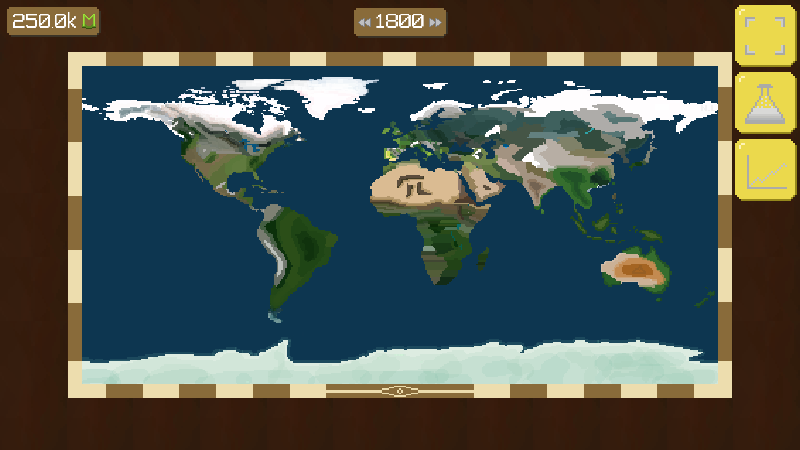
\includegraphics[width=\linewidth]{../images/worldView}
                \caption{Ecran principal du jeu}
                \label{fig:worldView}
        \end{figure} 
		
		\subsection{Les onglets du jeu} \label{onglets}
		Les menus du jeu sont affichés sous la forme d'onglets (qui représentent un journal).
		Il y a 3 onglets qui sont sous cette forme de journal: l'onglet de recherche, l'onglet des statistiques et l'onglet d'achat de centrales (ce dernier sera présenté dans la section \ref{regionView}).
		Tous les onglets sont construits sur le même modèle, seul leur contenu change. Ainsi, chaque onglet comporte un titre (en haut au centre), un bouton permettant de fermer l'onglet (en haut à droite), trois sections (au centre), un numéro de page (en bas au centre) et des flèches pour changer de page (en bas à gauche et à droite).
		
		
		\textbf{L'onglet de recherche} affiche les centrales énergétiques dans lesquelles le joueur peut investir des mondios (en appuyant sur le bouton vert où le prix de l'investissement est affiché) pour augmenter la probabilité qu'il les débloquera.
		
		\begin{figure}[H]
                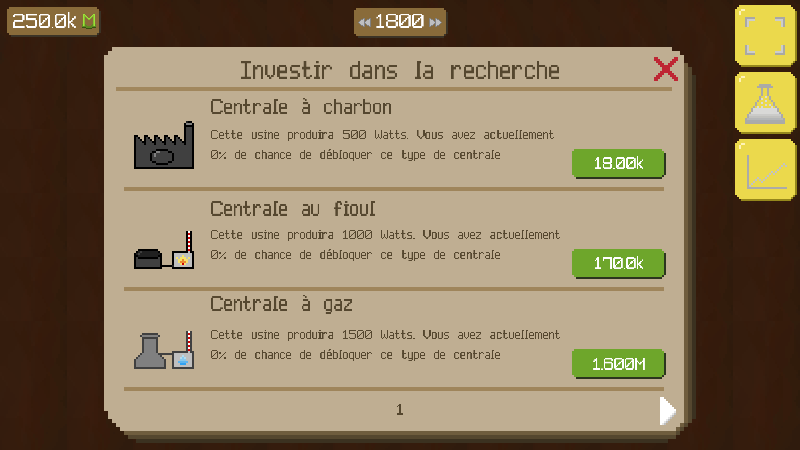
\includegraphics[width=\linewidth]{../images/recherche}
                \caption{Onglet de recherche}
                \label{fig:research}
        \end{figure}
        
        
        \textbf{L'onglet des statistiques} affiche les différentes statistiques de jeu. Ces informations indiquent servent à guider les choix du joueur. (Voir à chaque fois les figures \ref{fig:stats1} et \ref{fig:stats2}).
        \begin{itemize}
        		\item La première section concerne l'argent du joueur et sa production d'argent.
        		\item La seconde section affiche la production d'électricité des centrales du joueur.
        		\item La troisième section affiche l'émission totale de CO$_{2}$ depuis le début du jeu et l'émission hebdomadaire de CO$_{2}$ des centrales énergétiques.
        		\item La quatrième section (sur la deuxième page) affiche l'augmentation de température depuis le début de la révolution industrielle (début du jeu).
        \end{itemize}
        \begin{figure}[H]
                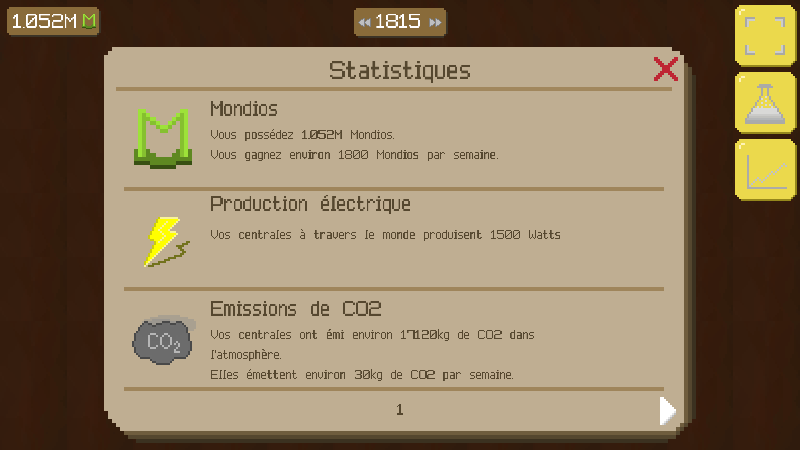
\includegraphics[width=\linewidth]{../images/stats1}
                \caption{Onglet des statistiques, première page}
                \label{fig:stats1}
        \end{figure}
        \begin{figure}[H]
                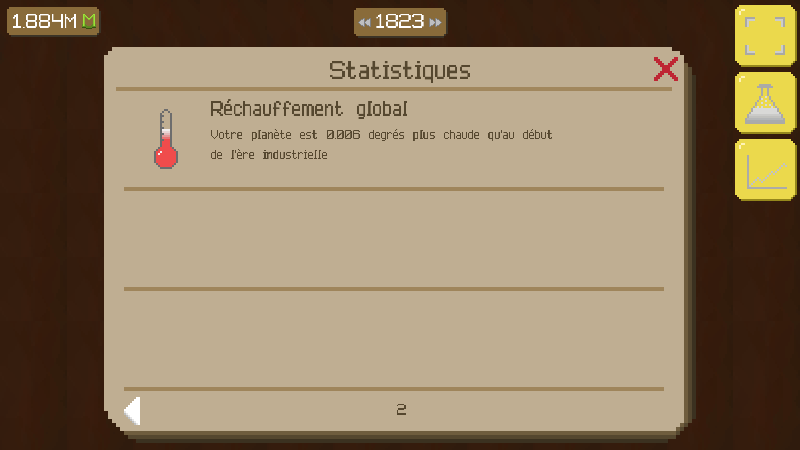
\includegraphics[width=\linewidth]{../images/stats2}
                \caption{Onglet des statistiques, deuxième page}
                \label{fig:stats2}
        \end{figure}
		
		\subsection{La vue des différentes régions} \label{regionView}
		En vue 'région', le joueur peut déverouiller des sites de production et interagir avec les centrales énergétiques construites (voir figure \ref{fig:region}).
		\begin{figure}[H]
                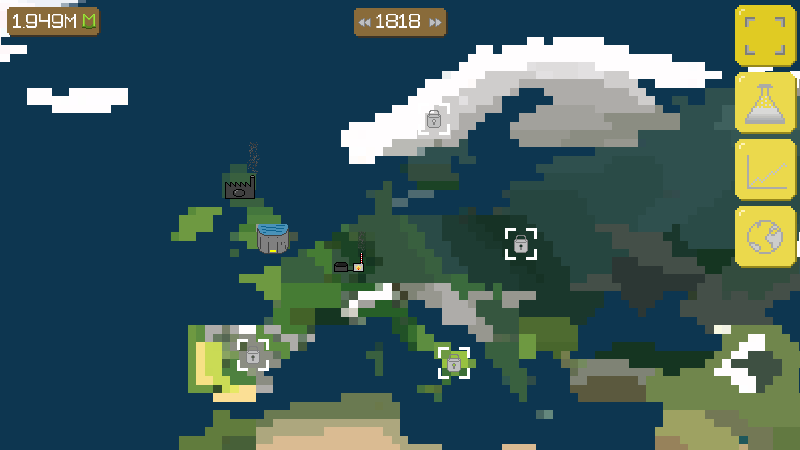
\includegraphics[width=\linewidth]{../images/region}
                \caption{La vue 'région'}
                \label{fig:region}
        \end{figure}
        
        En appuyant sur un site verouillé, une fenêtre de dialogue s'ouvre avec le prix du déverrouillage affiché (voir figure \ref{fig:unlockSite}).
        \begin{figure}[H]
                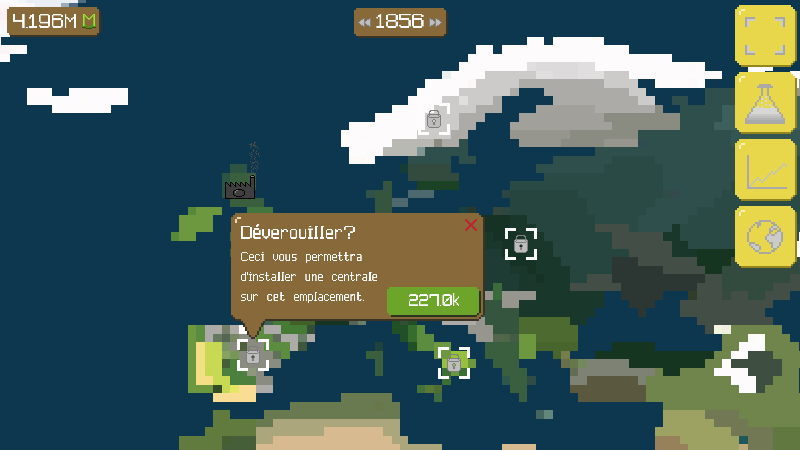
\includegraphics[width=\linewidth]{../images/unlockSite}
                \caption{Le déblocage d'un site de production}
                \label{fig:unlockSite}
        \end{figure}
        
        Il est ensuite possible de construire une centrale sur ce site de production (voir figure \ref{fig:buyPlant}).
        \begin{figure}[H]
                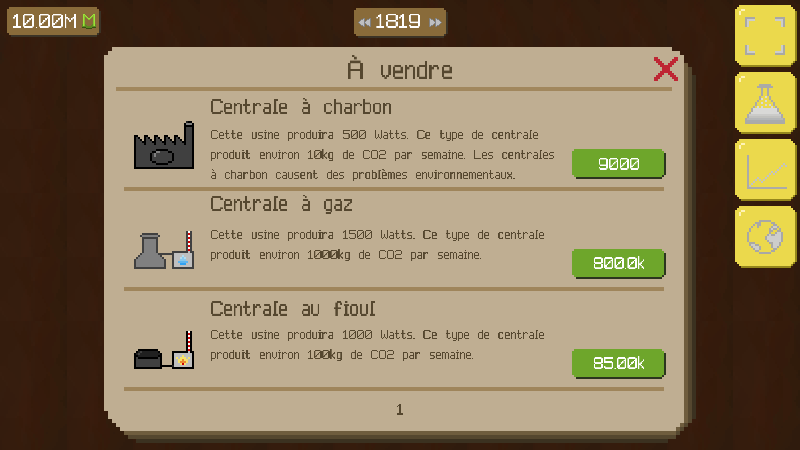
\includegraphics[width=\linewidth]{../images/buyPlant}
                \caption{L'achat d'une centrale électrique}
                \label{fig:buyPlant}
        \end{figure}
        
        
        Dans la vue 'région', on peut améliorer une centrale électrique pour qu'elle produise plus (ce qui aura comme conséquence qu'elle polluera également plus). Il est aussi possible de la détruire en appuyant sur le bouton rouge (voir figure \ref{fig:upgradePlant}).
        \begin{figure}[H]
                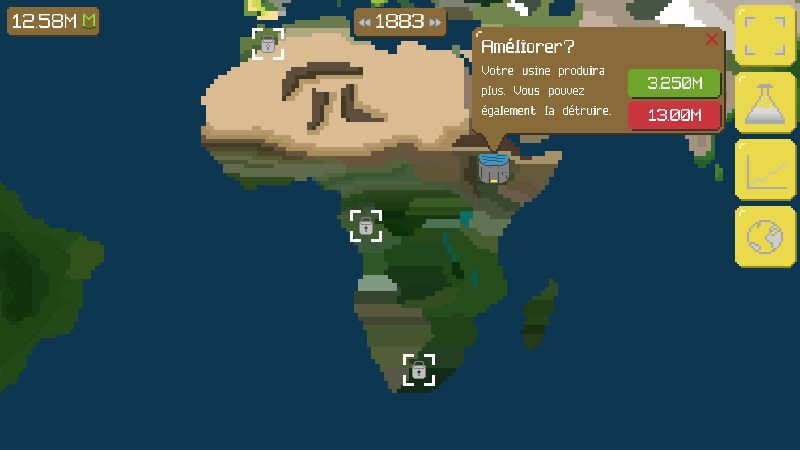
\includegraphics[width=\linewidth]{../images/upgradePlant}
                \caption{Amélioration d'une centrale électrique}
                \label{fig:upgradePlant}
        \end{figure}
        
        
        \subsection{Comment jouer}
        Le joueur commence par devoir choisir de jouer avec ou sans tutoriel (voir figure \ref{fig:mainMenu}).
        S'il choisit de suivre le tutoriel, il sera guidé dans le jeu par le personnage de Conseil qui lui expliquera le fonctionnement de tous les éléments du jeu et le but de la partie. 
        
        \begin{figure}[H]
                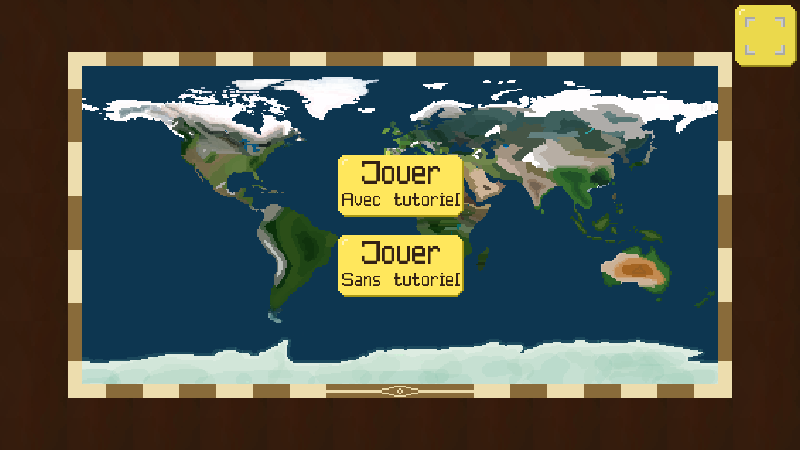
\includegraphics[width=\linewidth]{../images/mainMenu}
                \caption{Menu principal du jeu}
                \label{fig:mainMenu}
        \end{figure}
        
        Lorsqu'il commence une partie, le joueur possède \initMoney ~ Mondios. Il devra d'abord utiliser cet argent dans l'onglet 'Recherche' (voir figure \ref{fig:research}) qui lui permettra de débloquer une centrale énergétique. Après avoir suffisamment investi dans un type de centrale et attendu un certain moment (les centrales ne peuvent se débloquer qu'à chaque passage d'année), le type de centrale se débloque.
        
        
        Après avoir débloqué un type de centrale, le joueur peut se rendre dans une région (voir figure \ref{fig:region}) et déverrouiller un site de production (voir figure \ref{fig:unlockSite}). Après avoir déverrouillé le site de production, le joueur peut y construire une centrale énergétique (voir figure \ref{fig:buyPlant}). Cette centrale produira de l'énergie qui sera convertie en mondios et qui permettra d'investir dans la recherche d'autres centrales énergétiques ou de construire de nouvelles centrales. Il devra cependant faire attention à ne pas construire des centrales trop polluantes qui réchaufferaient sa planète de façon excessive (et qui lui ferait par conséquent perdre la partie).
        

        \section{Fonctionnement du code}
        Dans cette section, j'expliquerai quelles technologies j'ai utilisées pour créer mon jeu, comment les fichiers sont structurés et comment différentes parties du code fonctionnent. Je ne pourrai pas expliquer la totalité du code du jeu car cela serait trop long et n'apporterait pas grand chose à la compréhension du fonctionnement global du jeu. 
        
        \subsection{Les technologies utilisées}
        Le jeu a été crée dans le langage de programmation JavaScript (avec utilisation des dernières possibilités de ECMAScript 2016, voir la référence \cite{ecma2016}). La librairie open source Phaser JS en version 2.9.4 (voir la référence \cite{phaser}) m'a servi à simplifier certaines parties du code du jeu.
        
        
        \textit{Note : } Les commentaires dans les scripts présentés ci-dessous ne contiennent pas de caractères avec accent pour des soucis de compatibilité des caractères.
        
        
        \subsection{La structure des fichiers (voir annexe \ref{structure})}
        Les fichiers du jeu sont organisés en deux dossiers principaux: \textit{assets} et \textit{scripts}. Le dossier \textit{assets} contient tous les éléments visuels du jeu (c'est-à-dire les images et les animations). Le dossier \textit{scripts} contient tous les scripts du jeu. Les sous-dossiers de ce dossier sont \textit{classes, data, states} et \textit{utils}.
        
        
         \textit{Classes} contient toutes les définitions des classes utilisées dans le jeu. 
         
         
         \textit{Data} contient tous les scripts qui n'ont pas vraiment une action concrète mais qui servent à stocker des données du jeu (par exemple les valeurs de puissance et de production de CO$_{2}$ des centrales).
         
         
         \textit{States} contient tous les fichiers dans lesquels se trouvent les \textit{states} du jeu (voir la section \ref{main.js} pour une explication des \textit{states}).
         
         
         \textit{Utils} contient divers scripts qui sont utils à plusieurs endroits du jeu (par exemple le fichier \textit{globals.js}, voir la section \ref{globals.js} pour une explication).
        
       	
		\subsection{Le script d'entrée: main.js} \label{main.js}
		\lstinputlisting[language=JavaScript]{../../web_src/main.js}
		Ceci est le script principal car il lance l'exécution de toutes les autres parties du code.
		La variable \textit{config} définit plusieurs données utiles qui seront fournies à la classe \textit{Phaser.Game(\dots)} pour créer la variable \textit{game}. Cette variable est la variable principale de la librairie Phaser: chaque fois que l'on veut rajouter un élément de jeu (image, animation, bouton, etc\dots), que l'on veut démarrer un état du jeu (voir prochain paragraphe) ou que l'on veut modifier des propriétés de la caméra, c'est grâce à la variable \textit{game} qu'on le fera.
		
		
		Ensuite, les différents états du jeu (\textit{state}) sont définis. Chaque \textit{state} sert à définir un état du jeu. Le \textit{preloadState} représente par exemple l'étape où le jeu charge les éléments du jeu dans le cache du navigateur.
		Le \textit{mainMenuState} représente l'état du jeu lorsqu'on est dans le menu principal (voir figure \ref{fig:mainMenu}).
		Le premier paramètre de la méthode \textit{game.state.add(\dots)} est une chaîne de caractères qui représente la clé de l'état (grâce à laquelle on pourra démarrer plus tard cet état). Le second paramètre fait référence à un objet qui fera office de conteneur pour le state.
		
		
		Pour finir on appelle \textit{game.state.start("boot")} pour démarrer le boot state (pas très important pour la compréhension du fonctionnement global du jeu).
		
		\subsection{Les propriétés globales : globals.js} \label{globals.js}
		\lstinputlisting[language=JavaScript]{../../web_src/scripts/utils/globals.js}
		Ce script contient toutes les variables globales réutilisées durant tout le jeu. Il serait trop long de décrire l'utilité de toutes les propriétés et méthodes de l'objet \textit{globals}. C'est pourquoi je ne décrirai que certaines d'entre elles.
		
		\begin{itemize}
			\item \textit{initMoney} représente l'argent qu'a le joueur au départ du jeu.
			\item \textit{CO2Limit} représente la quantité maximum de CO$_{2}$ qu'il peut y avoir dans l'atmosphère. Passé cette limite, le joueur aura perdu la partie.
			\item \textit{globalWarmingLimit} représente la limite de réchauffement de la planète. Le réchauffement de la planète est calculé à partir de la quantité de CO$_{2}$ dans l'atmosphère.
			\item \textit{beginYear} et \textit{endYear} représentent les années de début et de fin du jeu.
			\item \textit{signals} est un objet qui contient les signaux utiles pour le tutoriel.
		\end{itemize}
		
		\subsection{Le fichier principal du jeu: game.js}
		\lstinputlisting[language=JavaScript]{../../web_src/scripts/states/game.js}
		La variable principale de ce fichier se nomme \textit{gameState}. C'est cette variable qui a été passée en argument de \textit{game.state.add(\dots)} dans le fichier main.js (voir section \ref{main.js}).
		
		\subsubsection{Les \textit{states} Phaser}
		Chaque \textit{state} dans Phaser est constitué de quatre méthodes principales: \textit{preload, create, update} et \textit{render}. 
		
		
		La méthode \textit{preload} sert à charger les éléments du jeu dans le cache du navigateur. Cependant, comme j'ai déjà chargé tous les éléments dont j'avais besoin dans ma \textit{state} appelée \textit{preload}, je n'ai plus besoin de le faire dans \textit{gameState}.  
		
		
		La méthode \textit{create} sert à exécuter des instructions qui ne doivent s'exécuter qu'une fois avant l'appel de la méthode \textit{update}.
		
		
		La méthode \textit{update} est appelée toutes les quelques millisecondes et permet d'effectuer des actions répétées.
		
		
		La méthode \textit{render} permet d'exécuter des méthode de débogage.
		
		\subsubsection{La méthode gameState.create}
		Le premier bloc de code dans cette section sert à mettre en place les différents éléments de l'interface: l'arrière-plan, la carte du monde et les autres éléments de l'interface utilisateur (UI).
		
		
		Ensuite, \textit{globReg.init()} permet d'initialiser les zones cliquables des régions de la carte et les sites de production des régions.
		
		
		Les prochaines lignes initialisent les différents \textit{managers}. Ceux-ci ont des fonctions importantes durant tout le jeu et gèrent plusieurs données importantes. Le \textit{moneyMgr} sert entre autre à stocker l'argent total possédé par le joueur et a une méthode qui permet de tester si on peut effectuer un achat d'une certaine valeur. \textit{productionMgr, timeMgr} et \textit{researchMgr} seront expliqués ci-après (voir respectivement les sections \ref{productionMgr}, \ref{timeMgr} et \ref{researchMgr}).
		
		
		On démarre ensuite le tutoriel si la variable \textit{globals.showTutorial} a la valeur \textit{true} (celle-ci a reçue la valeur vrai ou faux lors du clique sur le bouton du menu principal, voir figure \ref{fig:mainMenu}).
		
		\subsubsection{La méthode gameState.update}
		Dans cette méthode, la méthode \textit{globReg.update()} est appelée si il n'y pas d'instance de la classe \textit{Newspaper} active. \textit{globReg.update()} permet de constamment tester si le joueur a cliqué sur une des régions et d'enclencher le zoom sur cette région si c'est le cas.
		
		
		\subsection{Le gestionnaire de production: productionMgr.js} \label{productionMgr}
		\lstinputlisting[language=JavaScript, lastline=45]{../../web_src/scripts/classes/productionMgr.js}
		Le fichier productionMgr.js contient uniquement la classe ProductionMgr (la notation de classe telle qu'écrite ici est une nouvelle possibilité de ECMAScript 2015\footnote{Pour plus d'informations sur les classes, voir \url{https://developer.mozilla.org/fr/docs/Web/JavaScript/Reference/Classes}. Site consulté le 03.03.2018.}).
		
		\subsubsection{La méthode \textit{constructor}}
		La première méthode de n'importe quelle classe est la méthode \textit{constructor}. Celle-ci est appelée automatiquement lorsqu'on instancie un objet de cette classe. Ici,  plusieurs propriétés des instances de cette classe sont initialisées (le tiret bas devant les propriétés indiquent que celles-ci ne devraient normalement pas être accessibles depuis l'extérieur de l'instance de la classe). La propriété \textit{\_totPower} représente la puissance cumulée de toutes les centrales construites du jeu. \textit{\_CO2Production} représente la production de CO$_{2}$ totale des centrales. \textit{\_totCO2} représente la quantité totale de CO$_{2}$ émise depuis le début du jeu. \textit{\_powerToMondio} représente le taux de conversion de puissance à mondios (voir la section \ref{mondioProduction}).
		
		\subsubsection{La méthode \textit{update}}
		Les premières lignes servent à récupérer les données des sites de production pour pouvoir mettre à jour les propriétés \textit{\_totPower} et \textit{\_CO2Production}. 
		
		
		On augmente ensuite la valeur totale de l'argent du joueur et le total du CO$_{2}$ relâché dans l'atmosphère.
		
		
		Les prochaines lignes testent si la valeur totale de CO$_{2}$ excède le maximum de la valeur possible. Si c'est le cas, on démarre le \textit{state "gameEnd"} qui indique que la partie est perdue. On met également à jour l'opacité de la caméra pour avoir un écran de plus en plus sombre en fonction de la valeur de \textit{\_totCO2}.
		
		\subsubsection{La méthode \textit{get mondioProduction}} \label{mondioProduction}
		Cette méthode renvoie simplement la valeur de production de mondios utilisée dans la méthode \textit{update}. Elle utilise le mot-clé \textit{get} pour que la méthode agisse comme si c'était une propriété de la classe.
		
		\subsubsection{La méthode \textit{get globalWarming}} \label{globalWarming}
		Cette méthode renvoie la valeur du réchauffement global de la planète en \degree C. Elle dépend de la quantité totale de CO$_{2}$ dans l'atmosphère.
		
		\subsection{Le gestionnaire du temps: timeMgr.js} \label{timeMgr}
		\lstinputlisting[language=JavaScript, lastline=63]{../../web_src/scripts/classes/timeMgr.js}
		
		Cette classe définit le gestionnaire de la temporalité du jeu. J'expliquerai ici brièvement les méthodes principales de cette classe. Le gestionnaire de temps gère la mise à jour courte (qui dure 500ms de base et dans laquelle se produit par exemple la mise à jour de l'argent du joueur) et la mise à jour annuelle (qui lance par exemple le déblocage aléatoire des centrales énergétiques, voir section \ref{researchMgr}).
		
		\subsubsection{La méthode \textit{constructor}}
		Dans cette méthode je commence par définir des constantes de la classe. Les deux premières constantes définissent la durée de base d'une année. Ensuite j'indique l'échelle maximale et minimale de l'accélération ou du ralentissement du temps du jeu (modifié par les boutons à côté de l'affichage de l'année).
		
		
		J'assigne ensuite la valeur de la durée de l'année qui sera modifiée durant le jeu. Je crée ensuite une instance de \textit{Phaser.Timer} que j'assigne à \textit{this.\_timer}.
		
		%arrays et callbacks en italique ?
		Je crée ensuite les arrays qui contiendront les callbacks de la petite update (500ms de base) et de l'update annuelle. 
		
		
		Je définis ensuite la propriété \textit{\_year} qui contiendra l'année actuelle et une propriété \textit{\_lastYUSec} dont l'utilité sera expliquée plus tard.
		
		
		Enfin, je définis l'échelle de vitesse du temps qui pourra être modifiée par le joueur.
		
		\subsubsection{La méthode \textit{get \_delay}}
		Cette méthode renvoie la durée d'une petite update (cette méthode sera utilisée dans la méthode \textit{startUpdate}, voir section \ref{startUpdate}).
		
		\subsubsection{La méthode \textit{startUpdate}} \label{startUpdate}
		Cette méthode définit la boucle \textit{this.\_timerLoop} qui s'exécutera toutes les 500ms de base. Dans cette boucle on commence par appeler toutes les callbacks présentes dans \textit{this.\_callbacks}. 
		Pour savoir s'il y a un passage d'année, on teste si le compteur (en secondes) du timer est un multiple de la durée de l'année et si on ne vient pas de faire un passage d'année (d'où l'utilité de \textit{\_lastYUSec}). Si cette condition est vraie, on appelle \textit{this.\_yearUpdate}.
		On démarre ensuite le timer et l'affichage de l'année.
		
		\subsubsection{La méthode \textit{\_yearUpdate}}
		Dans cette méthode,  on commence par tester si l'année actuelle est plus grande (ou égale) à l'année de fin du jeu. Si c'est le cas, on fait un fondu vers un écran noir de la caméra et on démarre le \textit{state gameEnd} (qui est l'écran de fin du jeu).
		Si ce n'est pas le cas, on appelle toutes les callbacks de \textit{this.\_YUCallbacks}, on augmente la valeur de l'année et on met à jour l'affichage de l'année.
		
		\subsection{Le gestionnaire de recherche: researchMgr.js} \label{researchMgr}
		\lstinputlisting[language=JavaScript, lastline=53]{../../web_src/scripts/classes/researchMgr.js}
		
		Cette classe définit le fonctionnement de la recherche de centrales énergétiques.
		Chaque type de centrale a une probabilité de se débloquer (valant initialement 0) que le joueur peut augmenter en investissant dans la recherche de ce type de centrale. J'ai choisi \footnote{Suite à un conseil avisé de mon mentor.} d'utiliser une suite géométrique pour représenter la valeur de la probabilité car cela présentait l'avantage que la probabilité pourrait tendre vers 100\% mais ne jamais l'atteindre complètement (ce qui laisse une part de hasard).
		La valeur de la probabilité est une somme partielle d'une suite géométrique.
		\begin{align}
  			a_{k} &= c\cdot r^{k} \\
    			a_{0} &= c\cdot r^{0} = c \\
    			\sum_{k=0}^{\infty} a_{k} &= c\cdot \frac{1}{1-r} = 100 \\
    			r &= 1 - \frac{c}{100} < 1
		\end{align}
		% K COMMENCE À 0 OU 1 ???
		La première équation (1) correspond au terme général de la suite géométrique.
		La valeur de \textit{c} est égale au premier terme de la suite. Cela représente la valeur de la probabilité après le premier investissement et c'est donc cette variable que j'ai choisi de modifier pour obtenir différentes 'difficultés' de déblocage des centrales. Sachant que la valeur de la somme doit tendre vers 100 lorsque \textit{k} tend vers l'infini (3), je peux calculer la valeur de \textit{r} correspondante (4). Les formules sont tirées du \textit{Formulaires et tables}, p.90 (voir référence \cite{FetT}).
		
		%//la probabilite est une serie geometrique telle que
        %//a(k) = c*r^k
        %//a(0) = c*r^0 = c : premier terme de la serie => probabilite apres premier investissement
        %//et Sn quand n->+infiny
        %//Sn = c / (1-r) = 100
        
        \subsubsection{La méthode \textit{constructor}}
        Ici je définis les valeurs de \textit{c} de chaque type de centrale énergétique. Plus \textit{c} est grand, plus le type de centrale sera facile à débloquer. J'initialise ensuite les autres valeurs nécessaires au calcul de la suite géométrique $(r, k=0, partSum=0)$ grâce à la méthode \textit{\_setupUnlockData}. J'ajoute ensuite la méthode \textit{\_rndUnlockUpdate} aux mises à jour annuelles du gestionnaire du temps (cette méthode sera expliquée dans la section \ref{rndUnlockUpdate}).
        
        \subsubsection{La méthode \textit{increaseUnlockProb}}
        Cette méthode sert à augmenter la probabilité de débloquer une centrale. Elle est appelée depuis le \textit{newspaper} de recherche.
        Je commence par calculer le terme actuel de la série $a_{k}$ que j'ajoute à la somme partielle. J'augmente ensuite la variable \textit{k}. Je finis par mettre à jour l'affichage de la probabilité dans le \textit{newspaper} de recherche (grâce à la méthode \textit{gameEls.newspaper.softUpdate}).
        
        \subsubsection{La méthode \textit{\_rndUnlockUpdate}} \label{rndUnlockUpdate}
        Cette méthode est appelée à chaque mise à jour annuelle du gestionnaire du temps. Elle permet d'aléatoirement débloquer (ou non) une centrale énergétique. Je commence par parcourir tous les objets contenus dans \textit{unlockData}. Je génère ensuite un nombre rationnel aléatoire entre 0 et 100. Si le nombre aléatoire est plus petit que la probabilité de déblocage de la centrale, j'ajoute le titre de la centrale dans un array des noms de centrales débloquées pour pouvoir informer la joueur de quelles types de centrales il a débloquées. J'assigne ensuite la valeur \textit{-Infinity} à la probabilité pour que la centrale ne puisse pas être débloquée plusieurs fois. Je finis par appeler la méthode \textit{unlockFacType} qui s'occupe de débloquer le type de centrale.
        
        \section{Conclusion}
        \subsection{Ce que j'aurais aimé rajouter dans le jeu} \label{ajoutJeu}
		Par manque de temps, je n'ai pas pu ajouter toutes les possibilités que j'aurais voulu ajouter à mon jeu. J'expliquerai ici quelques-uns de ces ajouts.
		
		\subsubsection{Différents modes de difficulté}
		J'aurais voulu ajouter différents modes de difficulté pour que le jeu soit plus intéressant. J'aurais par exemple pu baisser la limite de CO$_{2}$ dans l'atmosphère avant la fin de la partie ou la probabilité de débloquer une centrale pour rendre le jeu plus difficile. J'aurais également voulu ajouter un besoin en énergie de la population qui aurait dû être satisfait, ce qui aurait rendu le jeu plus intéressant en forçant le joueur à construire plus de centrales tout en ne polluant pas trop l'atmosphère.
		
		\subsubsection{Possibilité de nouvelle partie après la fin du jeu}
		Une chose que j'avais prévu de faire était de pouvoir recommencer une partie après la fin du jeu sans devoir rafraîchir la page du navigateur. Cependant je me suis rendu compte que c'était plus compliqué que ce que j'imaginais (il fallait notamment réinitialiser plusieurs objets globaux).		
		
		\subsubsection{Musique et effets sonores}
		Afin de rendre le jeu plus agréable, j'aurais voulu ajouter une musique dans le jeu et des effets sonores (lors d'un clic sur un bouton par exemple). J'aurais notamment voulu ajouter la chanson \textit{Imagine} de John Lennon comme musique principale. 
		
		\subsubsection{Réalisme et évènements historiques}
		Il était originalement prévu que le jeu contienne des évènement historiques qui agissent sur le déroulement de la partie mais cela aurait demandé un investissement considérable en temps que je n'avais pas.
		J'aurais voulu ajouter également l'explosion aléatoire des centrales nucléaires à fission pour ajouter du réalisme au jeu. Un site de production sur lequel se trouvait une centrale nucléaire explosée aurait coûté très cher à nettoyer (et aurait donc été difficilement réutilisable).
		
		\subsubsection{Actions écologiques}
		Une fonctionnalité majeure du jeu (que j'avais d'ailleurs commencé à développer) aurait été un onglet avec différentes actions en faveur (ou en défaveur) de l'environnement. Le joueur aurait pu accepter d'investir dans des actions en faveur de l'environnement, ce qui aurait eu un impact sur le jeu (par exemple, une action en faveur de la préservation de la forêt amazonienne aurait diminué la quantité de CO$_{2}$ dans l'atmosphère).

				
		\subsection{Ce que m'a apporté ce travail de maturité}
		Ce travail de maturité m'a appris plusieurs choses par rapport à la programmation. J'ai notamment appris à organiser et structurer un code d'une taille importante en différents scripts, classes et méthodes. J'ai aussi l'impression d'avoir acquis de l'expérience pour ce qui est de prévoir comment concevoir le fonctionnement d'un morceau de code pour qu'il puisse être adaptable dans le futur.
		
		
		J'ai acquis également un certaine expérience dans la création de jeu vidéo (par exemple pour ce qui est de la création d'images et d'animations). Il a été également intéressant d'entendre l'avis de personnes ayant pu jouer à mon jeu. Certaines personnes m'ont fourni des critiques intéressantes grâce auxquelles j'ai parfois pu améliorer mon jeu.
		
		\subsection{Continuation du jeu}
		J'espère pouvoir continuer de développer mon jeu après l'avoir rendu dans cette version qui manque certaines fonctionnalités importantes (citées dans la section \ref{ajoutJeu}). Ce travail m'a grandement plu et j'aimerais beaucoup le continuer dans le but de peut-être un jour le diffuser à plus grande échelle que juste mon entourage afin de contribuer à transmettre le message de l'importance de l'écologie qui me tient à cœur.
        
        \newpage
        \begin{thebibliography}{9}

			\bibitem{phaser}
  			La librairie PHASER,
  			\url{http://phaser.io},
  			consulté le 6 septembre 2017.
  			
  			\bibitem{phaserDocs}
  			La documentation officielle PHASER,
  			\url{https://photonstorm.github.io/phaser-ce/},
  			consultée régulièrement jusqu'au 18 février 2018.
  			
  			\bibitem{ecma2016}
  			La version de JavaScript utilisée,
  			\url{https://en.wikipedia.org/wiki/ECMAScript#7th_Edition_-_ECMAScript_2016},
  			consulté le 28.02.2018.
  			
  			\bibitem{objsParis2100}
  			Les objectifs fixés par l'\textit{Accord de Paris sur le climat},
  			\url{https://fr.wikipedia.org/wiki/Accord_de_Paris_sur_le_climat#Objectifs},
  			consulté le 04.03.2018.
  			
  			\bibitem{FetT}
  			Commission Romande de Mathématiques, 
  			\textit{Formulaires et tables},
  			Éditions G d'Encre,
  			2015.
  			
  			\bibitem{font}
  			Police de caractère utilisée dans le jeu,
  			\url{https://www.searchfreefonts.com/font/advancedpixel-7.htm},
  			consulté le 23.09.2017.
  			
  			\bibitem{baseMap}
  			Image de base utilisée pour la carte de la terre (cette image a été modifiée),
  			\url{https://minecraftworld.files.wordpress.com/2011/05/earth_flat_map.jpg},
  			consulté le 06.09.2017.
 			
		\end{thebibliography}
		
		%\appendix
		\begin{appendices}
			\section{La structure des fichiers du jeu} \label{structure}
			\VerbatimInput{../structureFichiers.txt}
		\end{appendices}
\end{document}